\documentclass[a4paper, 11pt]{article}
\usepackage{covington}
\usepackage{amssymb}
\usepackage{amsmath}
\usepackage[catalan]{babel}
\usepackage{graphicx}
\usepackage{caption}
\usepackage{subcaption}
\usepackage{float}
\usepackage{bm}
\usepackage{layout}
\textheight=23.94cm 
\textwidth=17cm 
\topmargin=-1cm 
\oddsidemargin=-0.5cm 
 
\newcommand{\header}[4]{
	\begin{center}
		\rule{\linewidth}{0.5pt}
		
		{\small{#1}}
      
        \vspace{0.2in}
        
		{\large{#2}}
		
        \vspace{0.2in}
        
		{\small{#3}}
		
		\vspace{0.15in}
		
		{#4}
		
		\vspace{-0.1in}
		\rule{\linewidth}{0.6pt}
	\end{center}
}

\begin{document}
 
\header{\sc Barcelona Graduate School of Economics \hfill Master's Degree in Data Science}{\bf Statistical Modeling and Inference $-$ Project: Multiple Testing}{\sc Niti Mishra $\cdot$ Miquel Torrens $\cdot$ B\'alint V\'an}{November 2\textsuperscript{nd}, 2015}
Solution to proposed exercises.\\
%%%%%%%%%%%%%%%%
% PART 1
%%%%%%%%%%%%%%%%
% EXERCISE 1
\newline \textbf{\underline{Exercise 1.1}}\\
\newline Given $\alpha = 1 - F_H(c_\alpha)$, we have:
\begin{eqnarray}
F_H(c_\alpha) = 1 - \alpha \Leftrightarrow c_\alpha = F_{H}^{-1}(1- \alpha) \nonumber
\end{eqnarray}
Hence proved.\\
% EXERCISE 2
\newline \textbf{\underline{Exercise 1.2}}\\
\newline Given that $\mathbf{Y}$ is a dataset randomly drawn from a distribution truly consistent with $H$, we define the p-value by computing how likely is a test statistic drawn from $\mathbf{Y}$, meaning $T(\mathbf{Y})$, to be greater than a test statistic $T(\mathbf{X})$, given by a realisation of a random dataset $\mathbf{X}$ not necessarily consistent with $H$. That is:
\begin{eqnarray}
\text{p-value} = p(\mathbf{X}) = \mathbb{P}(T(\mathbf{Y}) > T(\mathbf{X})) \nonumber
\end{eqnarray}
We use the fact that $\alpha = 1 - F_H(c_\alpha)$ and that $\alpha = \mathbb{P}(T(\mathbf{Y}) > c_\alpha)$ to conclude that:
\begin{eqnarray}
1 - F_H(c_\alpha) = \mathbb{P}(T(\mathbf{Y}) > c_\alpha) \Leftrightarrow \mathbb{P}(T(\mathbf{Y}) > T(\mathbf{X})) = 1 - F_H(T(\mathbf{X})) \nonumber
\end{eqnarray}
Therefore, we find that $p(\mathbf{X})=1 - F_H(T(\mathbf{X}))$.\\
%\newline By construction, $T(\mathbf{X})$ is to $p(\mathbf{X})$ what $c_\alpha$ is to $\alpha$. We know that given $c_\alpha = F_{H}^{-1}(1- \alpha)$ we have $T(\mathbf{X}) = F_{H}^{-1}(1- p(\mathbf{X}))$. Then:
%\begin{eqnarray}
%1 - p(\mathbf{X}) = F_H(T(\mathbf{X})) \Leftrightarrow p(\mathbf{X}) = 1 - F_H(T(\mathbf{X}))\nonumber
%\end{eqnarray}
%Hence proved.\\
% EXERCISE 3
\newline \textbf{\underline{Exercise 1.3}}\\
\newline The CDF $F_Y(y)$ takes by definition values inside $[0, 1]$. Now we define $Z \equiv F_Y(y)$ and assume continuity on the CDF of $y$ and do:
\begin{eqnarray}
F_Z (z) = \mathbb{P}(F_Y(y) \leq z) = \mathbb{P}(y \leq F_Y^{-1}(z)) = F_Y(F_Y^{-1}(z)) = z \nonumber
\end{eqnarray}
Also for a uniform random variable\footnote{Note that in this proof $f_U = 1$ because it is a uniform distribution defined by parameters $a=0$ and $b=1$.} $U$ between 0 and 1:
\begin{eqnarray}
F_U (z) = \int f_U (u) du = \int_0^z 1 du = [u]_{0}^{z} = z - 0 = z \nonumber
\end{eqnarray}
For $z \in [0,1]$ we have $F_Z (z) = F_U (z)$ and as $Z = F_Y(y)$ we know that the distributions of $U$ and $F_Y(y)$ are the same.\\
\newline Given that the CDF gives $F_Y(y) \in [0,1]$, we know that also $1 - F_Y(y) \in [0,1]$. The identical proof can therefore be applied to $1 - F_Y(y)$ to find that it is also uniformly distributed.\\
% EXERCISE 4
\newline \textbf{\underline{Exercise 1.4}}\\
\newline We saw that $F_Y (y)$ and $1-F_Y (y)$ follow a uniform distribution regardless of the distribution of $Y$, as long as they are continuous. The p-value is defined as:
\begin{eqnarray}
p(\mathbf{X})=1 - F_H(T(\mathbf{X})) \nonumber
%\text{p-value} = \mathbb{P}(H < T(\mathbf{Y})) = F_H (T(\mathbf{Y})) \nonumber
\end{eqnarray}
We know that $F_H(T(\mathbf{X}))$ and therefore $1-F_H(T(\mathbf{X}))$ are continuous distributions and thus it is valid to apply the proof from Exercise 1.3 to say that the p-value follows a uniform distributuon.\\
%%%%%%%%%%%%%%%%
% PART 2
%%%%%%%%%%%%%%%%
% EXERCISE 1
\newline \textbf{\underline{Exercise 2.1}}\\
\newline Given that $y_i$ is uniform between 0 and 1 for all $i$, and given $\alpha \in [0,1]$, we know:
\begin{eqnarray}
\mathbb{P}(y_i < \alpha) = \alpha \nonumber
\end{eqnarray}
The complementary probability states\footnote{Recall that by continuity $\mathbb{P}(y_i = \alpha) = 0$.}:
\begin{eqnarray}
\mathbb{P}(y_i > \alpha) = 1 - \alpha \nonumber
\end{eqnarray}
Then:
\begin{eqnarray}
\mathbb{P}((y_1 > \alpha) \cap (y_2 > \alpha) \cap \dots \cap (y_m > \alpha)) = (1 -\alpha)(1 -\alpha) \dots (1 -\alpha) \nonumber
\end{eqnarray}
Where $(1 -\alpha)$ is replicated $m$ times. Then:
\begin{eqnarray}
\mathbb{P} \left(\bigcap_{i=1}^{m} y_i > \alpha \right) = (1-\alpha)^m \nonumber
\end{eqnarray}
Hence proved.\\
% EXERCISE 2
\newline \textbf{\underline{Exercise 2.2}}\\
\newline With a signle case the null hypothesis is accepted if the p-value $p_i(\mathbf{X}_i) > \alpha$. Thus the complete null is satisfied with probability:
\begin{eqnarray}
\mathbb{P} \left( \bigcap_{i=1}^{m} p_i(\mathbf{X}_i) > \alpha \right) \nonumber
\end{eqnarray}
We just proved that $\mathbb{P} \left(\bigcap_{i=1}^{m} y_i > \alpha \right) = (1-\alpha)^m$. So now we need to find the probability that at least in one of the cases the null hypothesis is rejected, and that is the complementary probability of the complete null. Thus, using $\mathbb{P}(A^c) = 1 - \mathbb{P}(A)$, we have:
\begin{eqnarray}
1 - \mathbb{P} \left(\bigcap_{i=1}^{m} p_i(\mathbf{X}_i) > \alpha \right) = 1 - (1-\alpha)^m \nonumber
\end{eqnarray}
Hence proved.\\
% EXERCISE 3
\newline \textbf{\underline{Exercise 2.3}}\\
\newline We need to find an expression for the case in which the complete null is satisfied $100 \times(1 - \alpha)$\% of the times, meaning that the overall type I error is $\alpha$. At that point, each independent test will be rejected $100 \times s$\% of the times, so we need to find an $s$ satisfying:
\begin{eqnarray}
\mathbb{P} \left( \bigcap_{i=1}^{m} p_i(\mathbf{X}_i) > s \right) = 1 - \alpha \nonumber
\end{eqnarray}
Then,
\begin{eqnarray}
(1-s)^m = 1 - \alpha \nonumber
\end{eqnarray}
And so, the probability of rejecting each independent test is:
\begin{eqnarray}
s = 1 - (1 - \alpha)^{1/m} \nonumber
\end{eqnarray}
Thus proved.\\
% EXERCISE 4
\newline \textbf{\underline{Exercise 2.4}}\\
\newline We plot for different values of $m$:
\begin{figure}[H]
\centering
\begin{subfigure}{.5\textwidth}
  \centering
  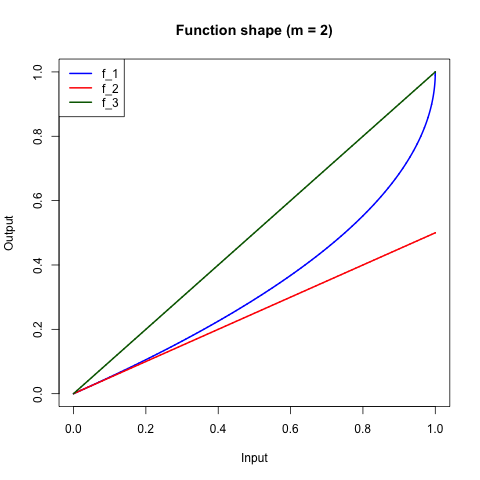
\includegraphics[width=1\linewidth]{pic2.png}
\end{subfigure}%
\begin{subfigure}{.5\textwidth}
  \centering
  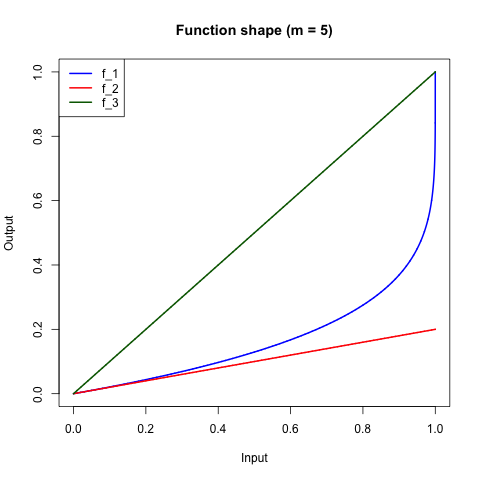
\includegraphics[width=1\linewidth]{pic3.png}
\end{subfigure}
\end{figure}
\begin{figure}[H]
\centering
\begin{subfigure}{.5\textwidth}
  \centering
  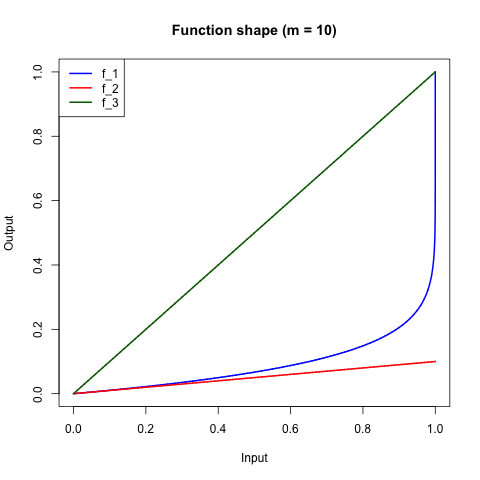
\includegraphics[width=1\linewidth]{pic4.png}
\end{subfigure}%
\begin{subfigure}{.5\textwidth}
  \centering
  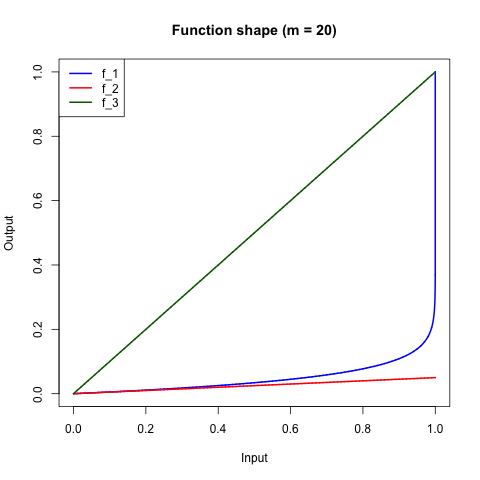
\includegraphics[width=1\linewidth]{pic5.png}
\end{subfigure}
\end{figure}
For $m=1$ the three curves overlap. We check graphically that $f_2 \leq f_1 \leq f_3$ for $\alpha \in [0,1]$.\\
% EXERCISE 5
\newline \textbf{\underline{Exercise 2.5}}\\
\newline We have $\alpha \in [0,1]$ and $m$ as a positive integer. We first prove that $f_2 \leq f_1$:
\begin{eqnarray}
\frac{\alpha}{m} \leq 1 - (1- \alpha)^{1/m} \nonumber
\end{eqnarray}
This would imply:
\begin{eqnarray}
(1-\alpha)^{1/m} \leq 1 - \frac{\alpha}{m} \nonumber
\end{eqnarray}
\newline It is straightforward to see that the inequality holds for $\alpha = 0$ and $\alpha=1$. To see if that is true for the all $\alpha \in [0,1]$, we want to check if the slope of the function on $\alpha$ is also steeper for $f_2$. We take derivatives on both sides with respect to $\alpha$:
\begin{eqnarray}
-\frac{1}{m} (1-\alpha)^{1/m -1} \leq -\frac{1}{m}  \Leftrightarrow (1-\alpha)^{1/m -1} \geq 1 \nonumber
\end{eqnarray}
These expressions are monotonic on  $\alpha$. The exponent on LHS in the right inequality is a negative number and $0<(1-\alpha)<1$, so the inequality holds. This concludes that $f_2 \leq f_1$ for $\alpha \in [0,1]$ and $m$ a positive integer.\\
\newline For $f_1 \leq f_3$ we need:
\begin{eqnarray}
1 - (1- \alpha)^{1/m} \leq \alpha \nonumber
\end{eqnarray}
We proceed analogously. This equality holds plugging $\alpha=0$ and $\alpha=1$. Derivatives on both sides should produce:
\begin{eqnarray}
\frac{1}{m} (1-\alpha)^{1/m -1} \leq 1 \nonumber
\end{eqnarray}
This holds with equality for $\alpha=0$ and is decreasing in $\alpha$, so with inequality for $\alpha>0$. Thus as a whole the inequality holds. Provided monotonicity, this concludes that $f_1 \leq f_3$.\\
\newline Hence, we conclude that $f_2 \leq f_1 \leq f_3$ for $\alpha \in [0,1]$ and $m$ a positive integer.\\
%\newline Notice that the RHS is increasing with respect to $m$ and LHS is decreasing with respect to $m$. For $m=1$, $\text{LHS}=\text{RHS} = 1-a$ and for $\lim_{m \rightarrow \infty} \text{LHS} = \lim_{m \rightarrow \infty} \text{RHS} = 1$. Hence with respect to $m$ the inequality holds.
% EXERCISE 6
\newline \textbf{\underline{Exercise 2.6}}\\
\newline An approach that makes no correction for multiple testing the level is determined by the size $\alpha \in [0,1]$. This level is, as proven before, necessarily higher than the one using a multiple-test sensitive approach, which leads to a significance level $1 - (1- \alpha)^{1/m}$.\\
%%%%%%%%%%%%%%%%
% PART 3
%%%%%%%%%%%%%%%%
% EXERCISE 1
\newline \textbf{\underline{Exercise 3.1}}\\
\newline We shall show this tackling separately both inequalities.\\
\newline As for the first inequality, the result of Exercise 2.2 concludes that:\begin{eqnarray}
\mathbb{P}_{C-H} \left[ \bigcup_{i=1}^{m} \left\lbrace p_i(\mathbf{Y}_i) < \alpha \right\rbrace \right] = 1 - (1-\alpha)^m. \nonumber
\end{eqnarray}
Given $\alpha \in [0,1]$ and $m$ as a positive integer, we know:
\begin{eqnarray}
(1-\alpha)^m \leq (1 - \alpha) \Leftrightarrow \alpha \leq 1 - (1-\alpha)^m \Leftrightarrow \alpha \leq \mathbb{P}_{C-H} \left[ \bigcup_{i=1}^{m} \left\lbrace p_i(\mathbf{Y}_i) < \alpha \right\rbrace \right] \nonumber
\end{eqnarray}
The second inequality is proved using Bonferroni's inequality\footnote{This inequality states that $\mathbb{P}(A_1 \cup A_2) = \mathbb{P}(A_1) + \mathbb{P}(A_2) - \mathbb{P}(A_1 \cap A_2) \leq \mathbb{P}(A_1) + \mathbb{P}(A_2)$, which can be generalized to $\mathbb{P}(\cup_i A_i) \leq \sum_i \mathbb{P}(A_i)$, also known as Boole's inequality.}. Given that the individual probability $\mathbb{P}_{C-H}(p_{i}(\mathbf{Y}_i) \leq \alpha) = \alpha$, then:
\begin{eqnarray}
\mathbb{P}_{C-H} \left[ \bigcup_{i=1}^{m} \left\{ p_i(\mathbf{Y}_i) < \alpha \right\} \right] &\leq& \sum_{i=1}^{m} \mathbb{P}_{C-H} (p_i(\mathbf{Y}_i) \nonumber \\
&\leq& \sum_{i=1}^{m} \alpha  \nonumber \\
&\leq& m \alpha \nonumber
\end{eqnarray}
Thus,
\begin{eqnarray}
\alpha \leq \mathbb{P}_{C-H} \left[ \bigcup_{i=1}^{m} \left\{ p_i(\mathbf{Y}_i) < \alpha \right\} \right] \leq m \alpha. \nonumber
\end{eqnarray}
%%%%%%%%%%%%%%%%
% PART 4
%%%%%%%%%%%%%%%%
% EXERCISE 1
\newline \textbf{\underline{Exercise 4.1}}\\
\newline If we define the event that all $y_i$ be greater than their respective $l_i$ as $A \equiv \cap_{i=1}^{m} \{y_i > l_i \}$, then we have $A^{c} = \cup_{i=1}^{m} \{y_i < l_i \}$, because that defines the event that at least some $y_i$ be smaller than its corresponding $l_i$. Since these are complementary probabilities,
\begin{eqnarray}
\mathbb{P} [ \cap_{i=1}^{m} \{y_i > l_i \} ] + \mathbb{P} [ \cup_{i=1}^{m} \{y_i < l_i \} ]  = 1\nonumber
\end{eqnarray}
This implies that for $\mathbb{P} [ \cap_{i=1}^{m} \{y_i > l_i \} ] = 1-\alpha$, we have:
\begin{eqnarray}
\mathbb{P} [ \cup_{i=1}^{m} \{y_i < l_i \} ] = 1 - (1-\alpha) = \alpha \nonumber
\end{eqnarray}
Now given that $p_{(i)}$ is uniformly distributed between 0 and 1, under the complete null hypothesis the probability that at least one $p_{(i)} < l_i$ is defined by:
\begin{eqnarray}
\mathbb{P}_{C-H} \left[ \bigcup_{i=1}^{m} \left\{p_{(i)} < \frac{i \alpha}{m} \right\} \right] = \alpha \nonumber
\end{eqnarray}
Hence proved.

\end{document}